\documentclass{Phyport}

\usepackage{placeins}
\usepackage{hyperref}
\hypersetup{
    colorlinks=true,
}

\exname{光的衍射} %实验名称
\extable{7}
\instructor{姚星星} %指导教师
\class{github} %班级
\name{MJ} %姓名
\stuid{2025} %学号

\nyear{2025} %年
\nmonth{11} %月
\nday{24} %日
\nweekday{一} %星期几

\begin{document}
\setcounter{page}{0}
\makecover

\section{预习报告（10分）}
\subsection{实验综述（5分）}

光的衍射是指光在传播过程中，遇到障碍物或者狭缝时，会偏离直线传播的路径而绕到障碍物后的现象，说明了光具有波动性。

光的衍射可以通过惠更斯-菲涅尔原理和傅里叶光学进行描述。根据惠更斯原理，每个衍射点都可以看作是一个次级波源，
波面由这些次级波源相干叠加而成，而各子波在空间某点的相干叠加就决定了该点波的强度。对光栅和狭缝的衍射现象进行分析时，通常采用波前的干涉与叠加原理。

对于单缝衍射，光强分布特征满足：
\[
    I = I_0 (\frac{\sin \mu}{\mu})^2
\]

衍射角度满足：
\[
    a \sin \theta = m \lambda , \quad m = \pm 1, \pm 2, \pm 3, \cdots
\]

对于双缝衍射，衍射条纹由两条狭缝产生的波的干涉形成，亮条纹的位置满足：
\[
    d \sin \theta = m \lambda , \quad m = \pm 1, \pm 2, \pm 3, \cdots
\]  

实验前，预先调节光路与光学元件位置，确保激光光束通过准直器或聚焦镜准直，各元件共轴，整体精度和稳定性较高。
实验时，通过改变衍射物的形状和尺寸，观察到不同形状的衍射物产生不同的衍射光强分布；使用一维光栅，测量±1级衍射点的间距并结合光栅的周期，
计算出光源的波长；使用单缝，测量不同衍射级次衍射条纹的位置并计算单缝的宽度，同时通过光电流测量不同位置的光强，验证不同级次光强之间的比例关系。
在实验中可以观察到不同的衍射现象，并且中心光强最大，其他级次的光强随衍射角度增大而逐渐减弱，基本符合波动光学理论。


\subsection{实验重点（3分）}

本实验的学习重点在于理解光的衍射现象和规律，尤其是不同形状衍射物的衍射光强分布特征和二维光栅衍射的特征，
以及掌握利用光的衍射法测量微小量的方法。


\subsection{实验难点（2分）}

本实验的实现难点主要在于精确调节光路和测量衍射图案上。光学元件必须确保精确共轴，以及衍射条纹较为微小，
需要精确测量衍射点间的距离。另外，要准确辨认衍射图案中的各个光强级次，避免误读或计算错误。


\newpage
\section{原始数据（20分）}
\begin{figure}[htbp!]
    \centering
    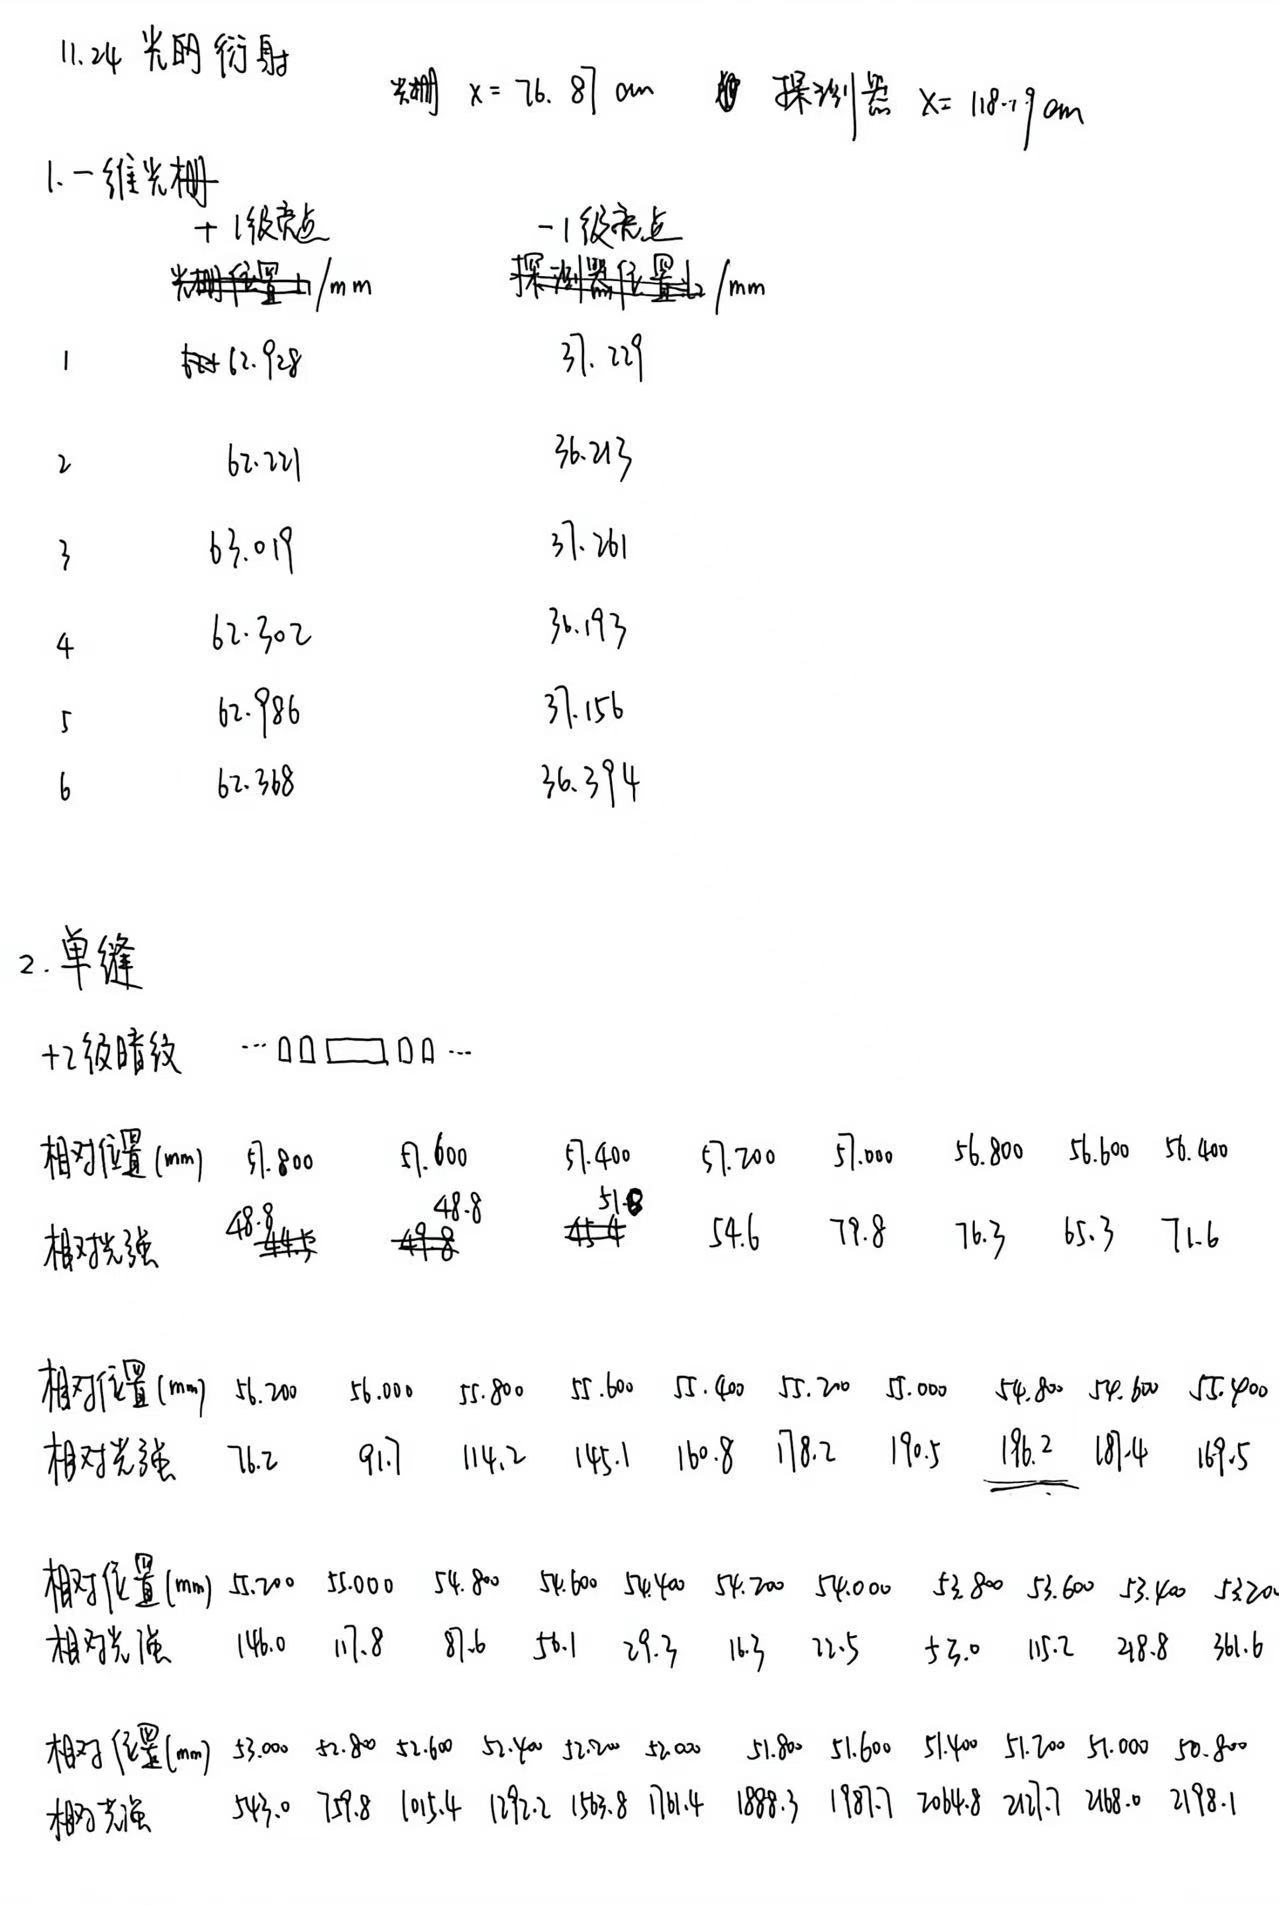
\includegraphics[width=0.8\textwidth]{data1.jpg}
\end{figure}

\FloatBarrier

\begin{figure}[htbp!]
    \centering
    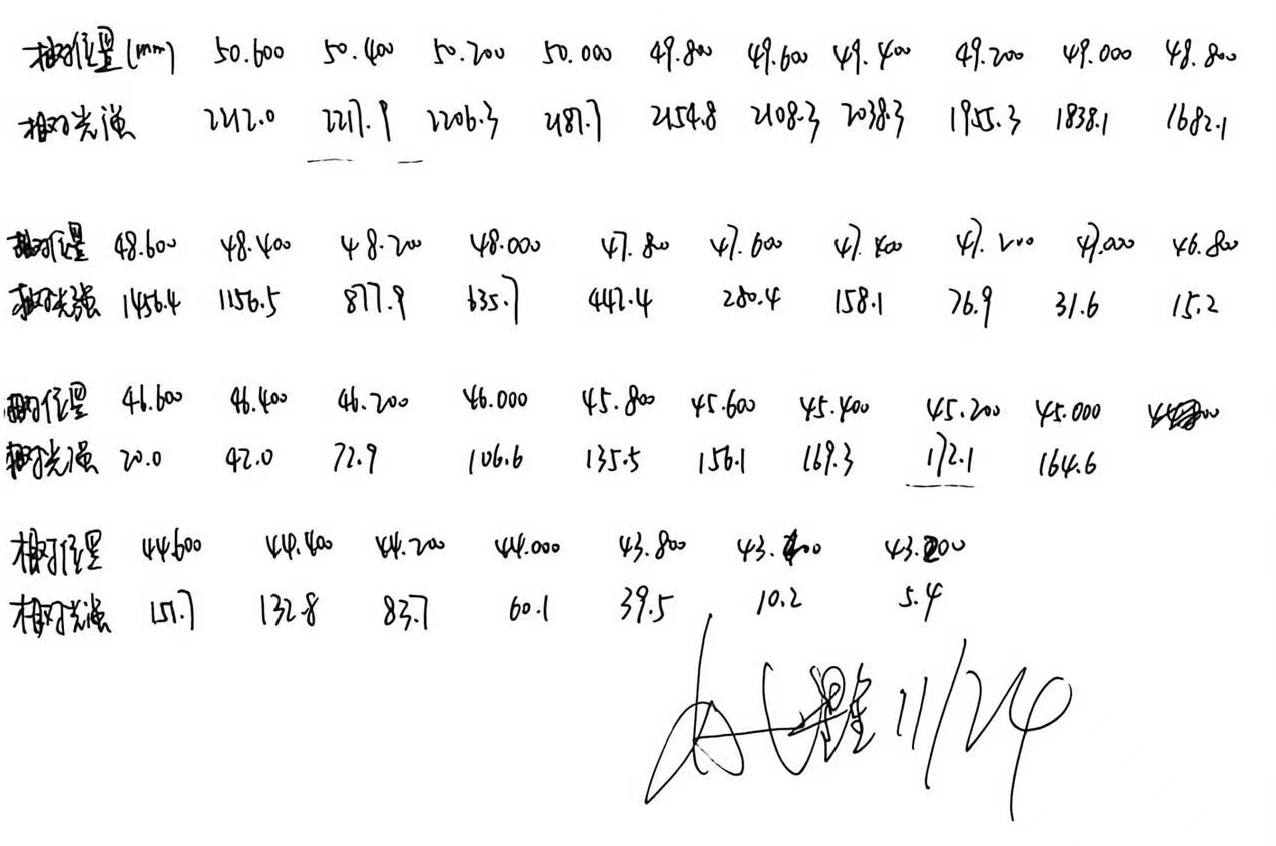
\includegraphics[width=0.8\textwidth]{data2.png}
\end{figure}

\FloatBarrier

\section{结果与分析（60分）}
\subsection{数据处理与结果（30分）}

\textbf{1.一维光栅衍射}

多次测量 $\pm 1$ 级衍射点间距离，其中光栅位置 $L_1 = 768.7 mm$ ，探测器位置 $L_2 = 1181.9 mm$

\begin{table}[htbp!]
    \centering
\begin{tabular}{|l|l|l|l|}
    \hline
    次数 & $+1$ 级亮点位置 $x_{+1} (mm) $ & $-1$ 级亮点位置 $x_{-1} (mm) $ & $\Delta x = x_{+1} - x_{-1} (mm)$ \\
    \hline
    1 & 62.928 & 37.229 & 25.699 \\
    \hline
    2 & 62.221 & 36.213 & 26.008 \\
    \hline
    3 & 63.019 & 37.261 & 25.758 \\
    \hline
    4 & 62.302 & 36.193 & 26.109 \\
    \hline
    5 & 62.986 & 37.156 & 25.830 \\
    \hline
    6 & 62.368 & 36.394 & 25.974 \\
    \hline
\end{tabular}
\end{table}

根据光栅方程可以计算出光源波长：
\[
    (a + b) \sin \theta = \pm \lambda , \quad a + b = 0.02 mm  
\]

结果为：

\begin{table}[htbp!]
    \centering
    \begin{tabular}{|c|c|c|c|c|c|c|}
        \hline
        实验 & $\lambda_1$ & $\lambda_2$ & $\lambda_3$ & $\lambda_4$ & $\lambda_5$ & $\lambda_6$ \\
        \hline
        波长 $(nm)$ & 622 & 630 & 624 & 630 & 626 & 628 \\
        \hline
    \end{tabular}
\end{table}

\FloatBarrier

六次测量的平均波长为：
\[
\bar{\lambda} = \frac{1}{6} \sum_{i=1}^6 \lambda_i = 626 nm
\]

计算波长的不确定度时，包括重复测量导致的 $A$ 类不确定度：
\[
u_A(\lambda) = \sqrt{\frac{1}{n(n-1)} \sum_{i=1}^{n} (\lambda_i - \bar{\lambda})^2} = 1.37 nm , \quad n = 6
\]

和仪器本身允差造成的 $B$ 类不确定度：
\[
u_B(\lambda) = \sqrt{ (\Delta_{\text{导轨}} L \frac{d \lambda}{d \Delta x})^2 + (\Delta_{\text{手轮}} L \frac{d \lambda}{d \Delta x})^2 } = 12.1 nm
\]

总不确定度为：
\[
u(\lambda) = \sqrt{u_A^2 + u_B^2} = 12.1 nm
\]

最终得到光源波长为：
\[
\lambda = \bar{\lambda} \pm u(\lambda) = 626.0 \pm 12.1 nm
\]

与波长标准值 $\lambda_0 = 650.0 nm$ 的相对误差为：
\[
E = \frac{|\lambda - \lambda_0|}{\lambda_0} \times 100 \% = 3.69 \%
\]

\textbf{2.单缝衍射}

记录 $\pm 2$ 级暗纹间的数据

\begin{table}[htbp!]
    \centering
\begin{tabular}{|l|l|l|l|l|l|l|l|l|l|}
    \hline
    相对位置 & 43.200 & 43.400 & 43.800 & 44.000 & 44.200 & 44.400 & 44.600 & 45.000 & 45.200 \\
    相对光强 & 5.4 & 10.2 & 39.5 & 60.1 & 83.7 & 132.8 & 151.7 & 164.6 & 172.1 \\
    \hline
    相对位置 & 45.400 & 45.600 & 45.800 & 46.000 & 46.200 & 46.400 & 46.600 & 46.800 & 47.000 \\
    相对光强 & 169.3 & 156.1 & 135.5 & 106.6 & 72.9 & 42.0 & 20.0 & 15.2 & 31.6 \\
    \hline
    相对位置 & 47.200 & 47.400 & 47.600 & 47.800 & 48.000 & 48.200 & 48.400 & 48.600 & 48.800 \\
    相对光强 & 76.9 & 158.1 & 280.4 & 442.4 & 635.7 & 877.9 & 1156.5 & 1456.4 & 1682.1 \\
    \hline
    相对位置 & 49.000 & 49.200 & 49.400 & 49.600 & 49.800 & 50.000 & 50.200 & 50.400 & 50.600 \\
    相对光强 & 1838.1 & 1955.3 & 2038.3 & 2108.3 & 2154.8 & 2187.7 & 2206.3 & 2217.9 & 2212.0 \\
    \hline
    相对位置 & 50.800 & 51.000 & 51.200 & 51.400 & 51.600 & 51.800 & 52.000 & 52.200 & 52.400 \\
    相对光强 & 2198.1 & 2168.0 & 2127.7 & 2064.8 & 1987.7 & 1888.3 & 1761.4 & 1563.8 & 1292.2 \\
    \hline
    相对位置 & 52.600 & 52.800 & 53.000 & 53.200 & 53.400 & 53.600 & 53.800 & 54.000 & 54.200 \\
    相对光强 & 1015.4 & 759.8 & 543.0 & 361.6 & 218.8 & 115.2 & 53.0 & 22.5 & 16.3 \\
    \hline
    相对位置 & 54.400 & 54.600 & 54.800 & 55.000 & 55.200 & 55.400 & 55.600 & 55.800 & 56.000 \\
    相对光强 & 29.3 & 56.1 & 87.6 & 117.8 & 146.0 & 169.5 & 187.4 & 196.2 & 190.5 \\
    \hline
    相对位置 & 56.200 & 56.400 & 56.600 & 56.800 & 57.000 & 57.200 & 57.400 & 57.600 & 58.600 \\
    相对光强 & 178.2 & 160.8 & 145.1 & 114.2 & 91.7 & 76.2 & 71.6 & 65.3 & 48.8 \\
    \hline
\end{tabular}
\end{table}


使用MATLAB绘制 $\pm 2$ 级暗纹间的图案，并标出0级最大光强和 $\pm 1$ 级最大光强的位置：
\begin{figure}[htbp!]
    \centering
    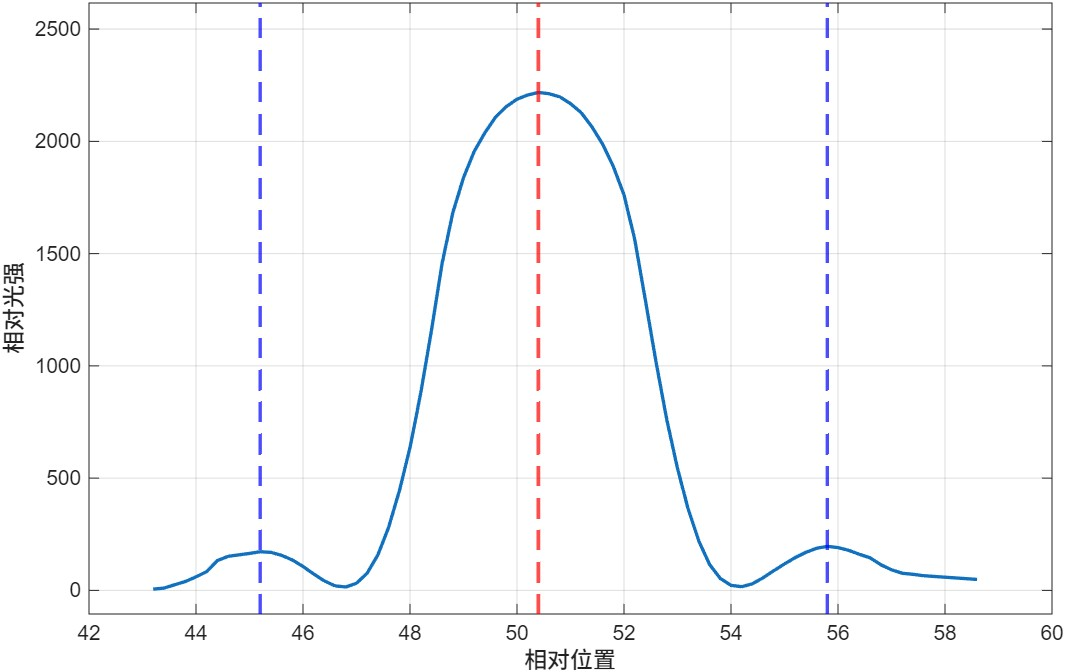
\includegraphics[width=0.6\textwidth]{part2demo.jpg}
\end{figure}

\FloatBarrier

并且根据 $\pm 1$ 级亮纹中心位置方程计算单缝宽度：
\[
a = 1.43 \frac{\lambda}{\sin \theta} = 0.075 mm
\]

验证正一级明纹和中心明纹的光强比：
\[
\frac{I_{+1}}{I_0} = \frac{172.1}{2217.9} = 7.75 \%
\]

验证负一级明纹和中心明纹的光强比：
\[
\frac{I_{-1}}{I_0} = \frac{196.2}{2217.9} = 8.84 \%
\]

光强比偏离 $4.7 \%$ 和两边光强不一致的原因将分别在误差分析和思考题部分给出。

\subsection{误差分析（20分）}

对于一维光栅的衍射实验部分，测量得到的光源波长的 $A$ 类不确定度相对小，说明实验测量过程比较稳定，
而仪器误差较大，最终光源波长的测量结果和标准值的相对误差在 $4 \%$ 以内，说明总体测量较为准确，那么主要误差可能来自：
\begin{enumerate}
    \item 激光器、光栅、探测器无法完全共轴，衍射图案会有偏移，导致衍射图案位置测量误差；
    \item 通过光电流来判断亮纹中心时，读数很难稳定，导致位置判断产生误差；
    \item 在测量探测器位置时，主轴和手轮的读数都有误差，会放大为波长的误差；
    \item 光栅可能刻线损伤或者沾污，导致衍射角偏移，产生误差。
\end{enumerate}

对于单缝衍射实验部分，测量得到的正负一级明纹和中心明纹光强比要大于理论值，
主要可能是：
\begin{enumerate}
    \item 探测器在强光区域可能产生饱和或响应压缩，中心光强受到的影响最大；
    \item 实验环境的背景光、探测器暗电流噪声等都会干扰衍射光线，导致光强比误差；
    \item 在测量探测器位置时产生的误差放大，导致光强比的误差。
\end{enumerate}

\subsection{实验探讨（10分）}

本实验观察了不同形状孔径及单缝的衍射现象，直观了解了中央亮纹最强、两侧亮纹逐渐减弱的规律，
并具体计算了一维光栅的光源波长和单缝宽度，以及测量单缝衍射光强分布图形。

\section{思考题（10分）}

\textbf{1. 单缝衍射两侧光强不是严格对称的原因是什么？}

理论上，理想的单缝在均匀照明、狭缝厚度一致、边缘完全平直且入射光为完全平面波的条件下，
衍射图样应该左右严格对称。但在实际实验中，两侧光强不完全对称，原因主要包括：
\begin{enumerate}
    \item 狭缝宽度不均匀，并且边缘不是完全平直，导致两侧光强不对称；
    \item 入射光不是严格的平面波或不完全均匀，本身就具有不对称性；
    \item 调整光栅和探测器时，无法使得光线完全垂直入射，导致衍射图案产生偏移；
    \item 环境中的背景光、光路上空气折射率的波动，都可能引起衍射图案的偏差。
\end{enumerate}

\textbf{2. 狭缝宽度是否越小越好，为什么？}

理论上减小狭缝宽度可以使衍射现象更加明显，但是实验中狭缝宽度并不是越小越好，
必须综合考虑测量、误差等因素。

首先，根据单缝衍射公式
\[
a \sin \theta = m \lambda
\]
当狭缝宽度 $a$ 非常小的时候，衍射角接近 90°，较难形成方便测量的条纹结构。

其次，狭缝过窄时，光经过狭缝后的能量显著减弱，衍射图案亮度降低，
探测器难以测量微弱的光强；并且这时衍射后的光强还很容易受到环境干扰，
造成较大的误差。

因此，要选择适当宽度的狭缝，保证衍射明显并且光强稳定。

\textbf{3. 描述一个生活光的衍射现象，怎么做？现象是什么？}

将灯光通过手指缝隙照向墙面，可以看到中央亮纹最亮、两侧出现逐渐减弱的条纹结构。
这是因为手指之间形成狭缝，光在边缘发生衍射并相互干涉，形成明暗相间的花样，直观展示了光具有波动性。

\begin{thebibliography}{9}
    \bibitem{ref1}
    刘秋武,张庆. 单缝衍射光强分布的异常分析[J]. 实验室科学,2010,13(1):183-185. DOI:10.3969/j.issn.1672-4305.2010.01.066. 

    \bibitem{ref2}
    王致远,范玲. 半波带法计算夫琅禾费单缝衍射各级明纹中心相对光强[J]. 大学物理,2024,43(8):68-71. DOI:10.16854/j.cnki.1000-0712.230274.
    
    \bibitem{ref3}
    延安. 用手电筒演示光的衍射[J]. 课程教育研究,2013(10):182-182,183. DOI:10.3969/j.issn.2095-3089.2013.10.172. 

\end{thebibliography}

\input{注意事项}
\end{document}
